\section{Results} \label{sec:results}
Our first validation experiment on synthetic data was preformed as such: First we choose 50\% of the tips of a phylogeny and censored those dates, we next used root-to-tip regression \citep{APE} on the remaining data to calibrate the molecular clock for the tree. Finally, for each censored date, we reconstructed the expected date using the expected number of substitutions.

In all of our experiments, before any analysis is done, all times are re-scaled to lie between $0$ and $1$. This is calculated as $$ \text{new time} = \frac{\text{time} - \text{min time}}{\text{max time} - \text{min time}}$$ this gives normalized time. Errors are then calculated from this number, which we call normalized error. On the left figure \ref{fig:results1} shows a linear regression over either simulation time or time from a reference point (for patient data). On the right side of figure \ref{fig:results1}, is the superposition of an error density estimate for each data set within a category. 


\begin{figure*}[!ht] \label{fig:results1}
	\centering
	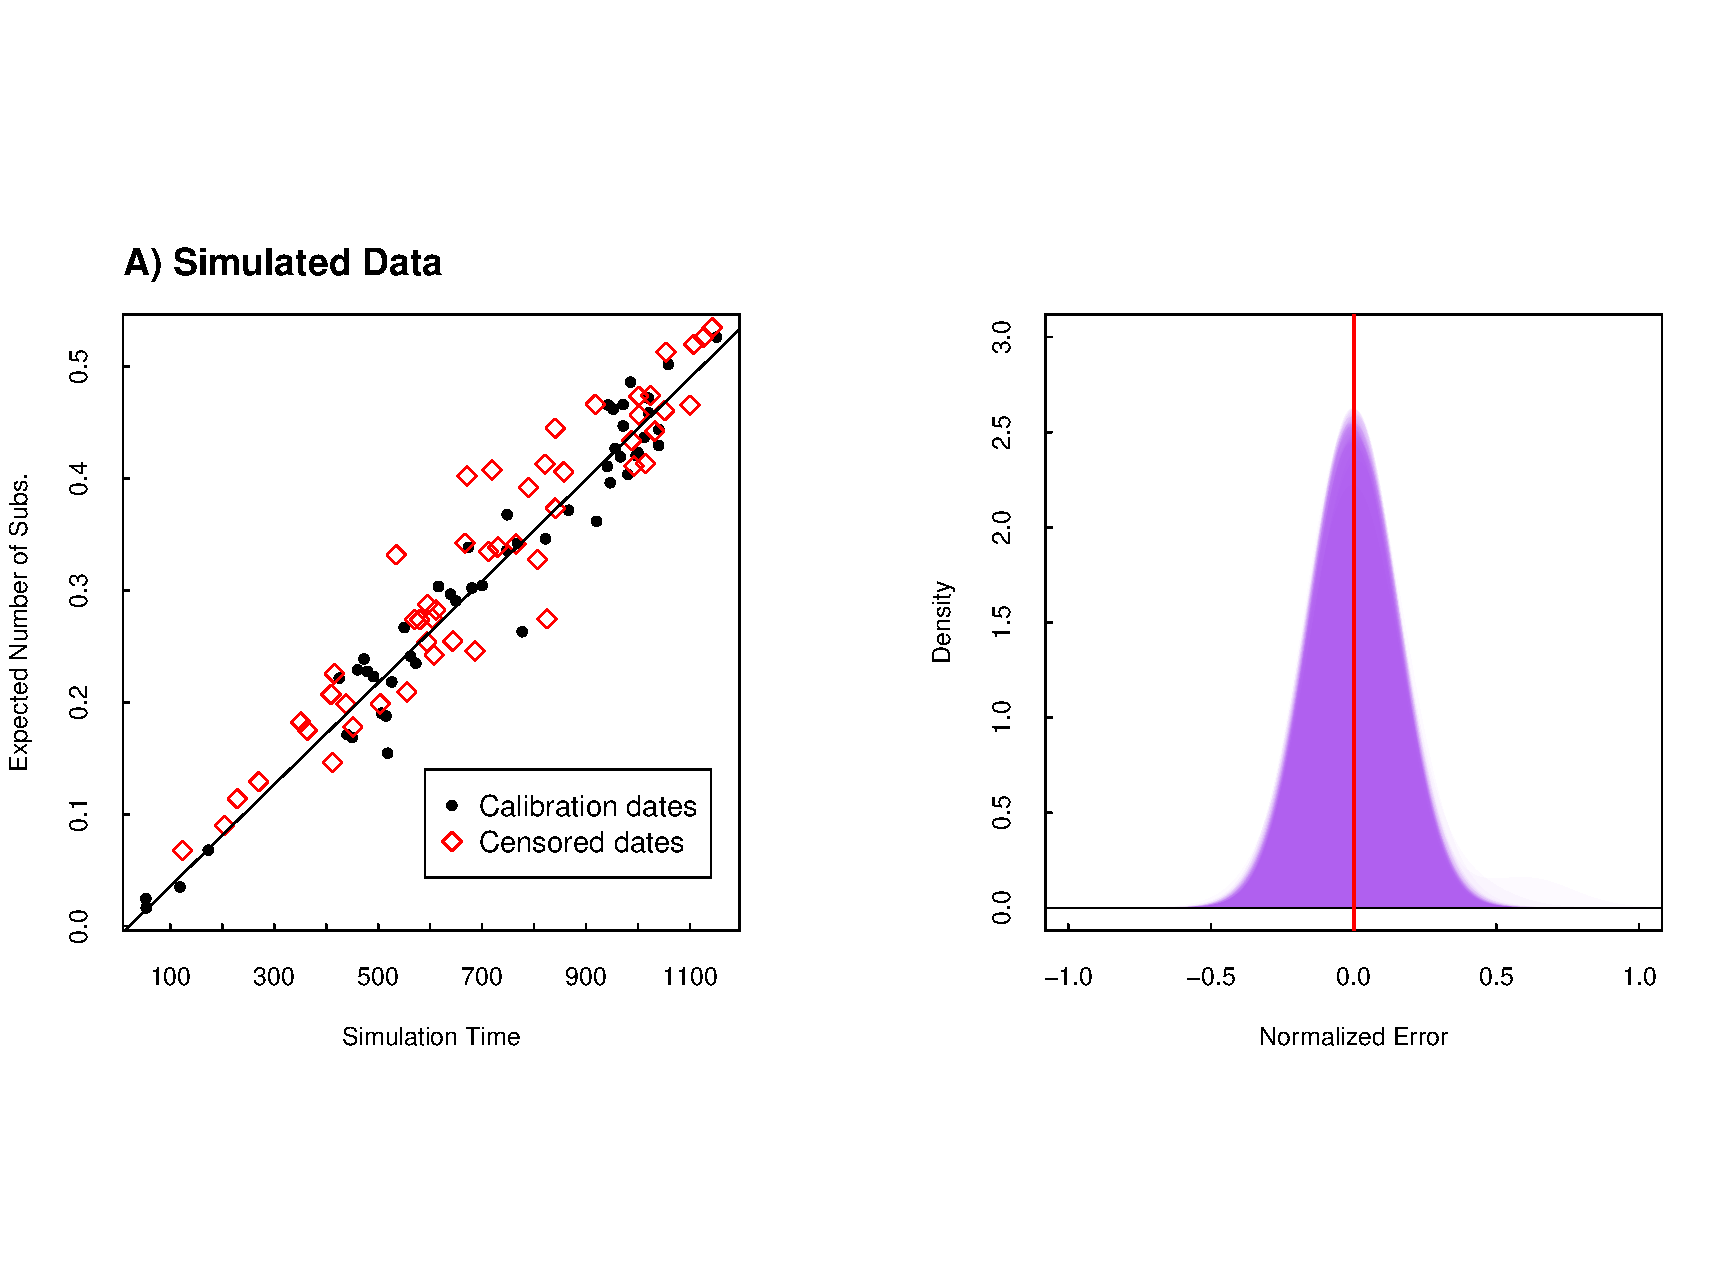
\includegraphics[trim=0cm 0cm 0cm 6cm, clip=true, scale=0.425]{figures/simulated.pdf} \\
	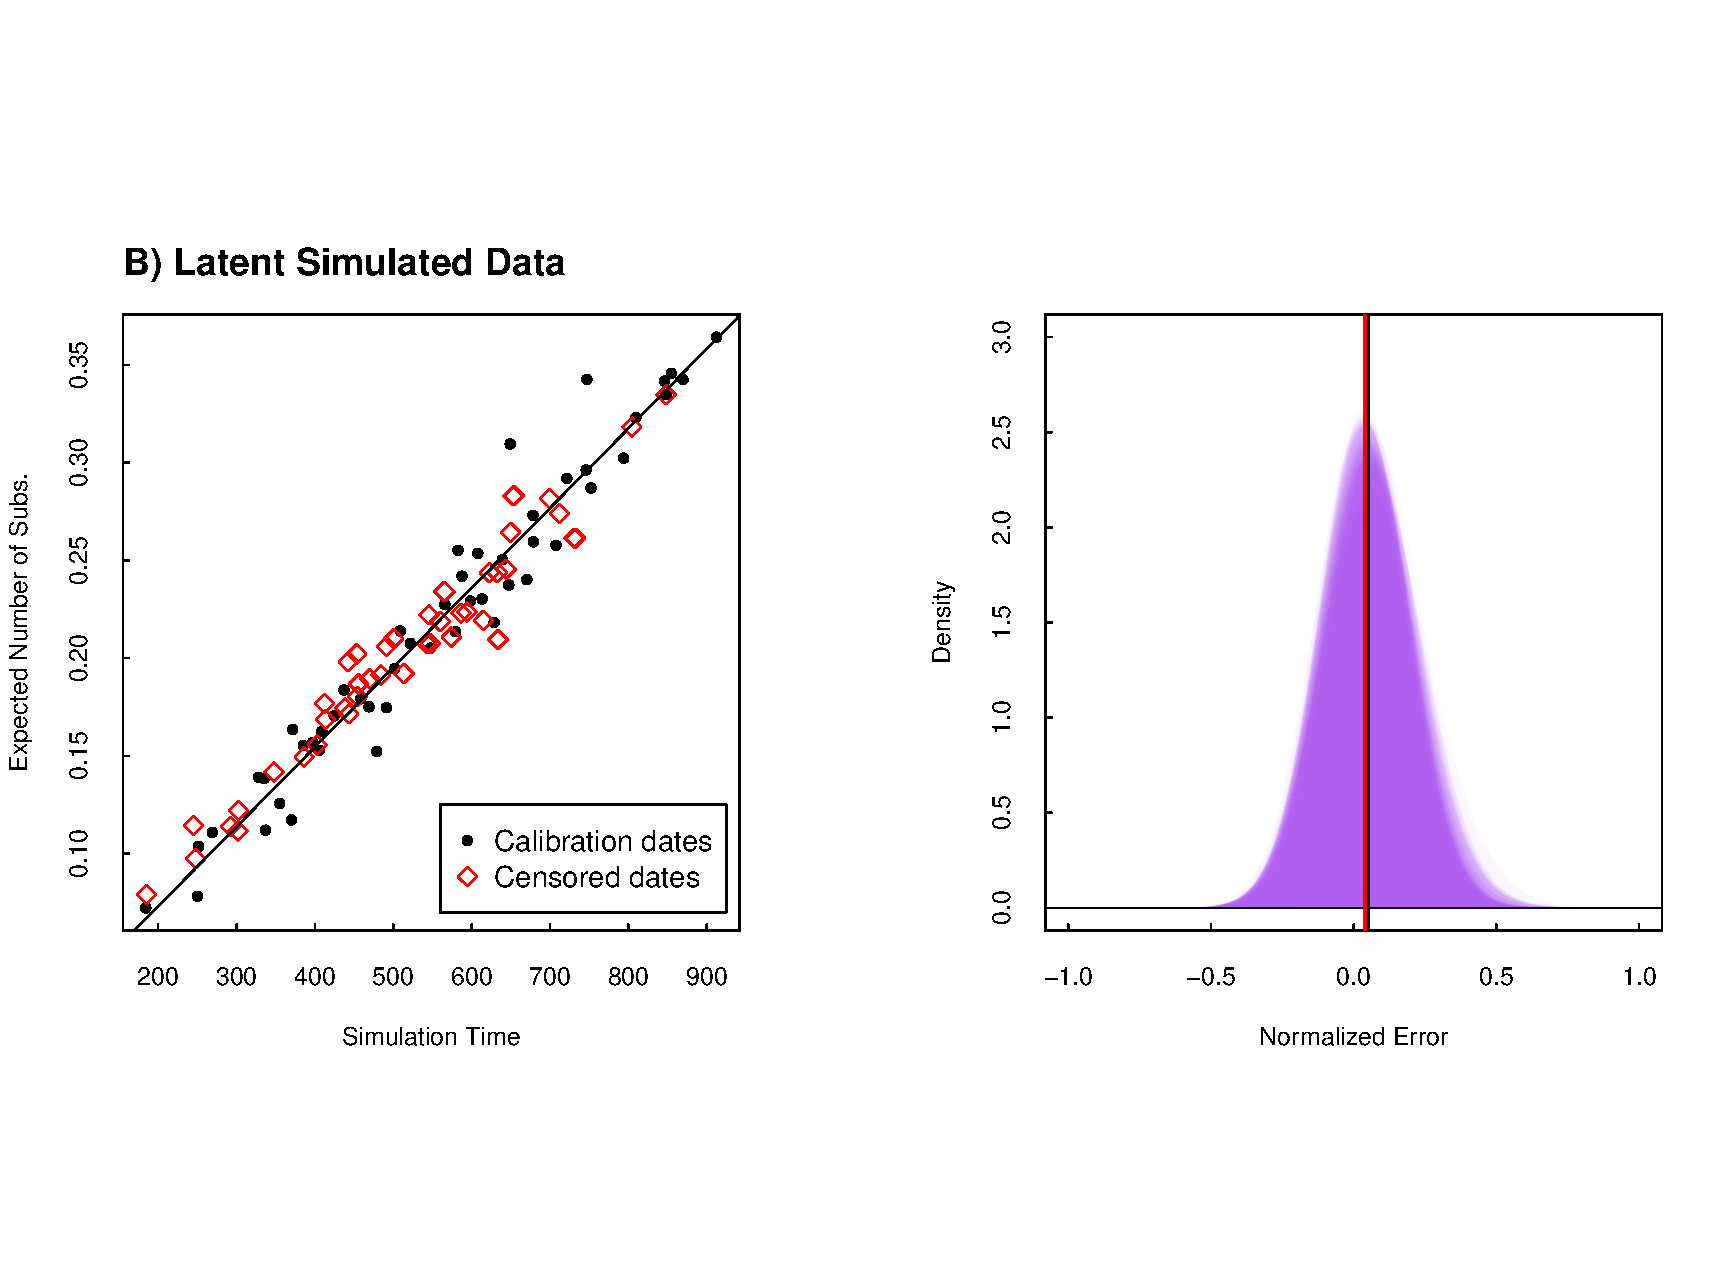
\includegraphics[trim=0cm 0cm 0cm 7cm, clip=true,scale=0.425]{figures/simulated_latent.pdf}\\
	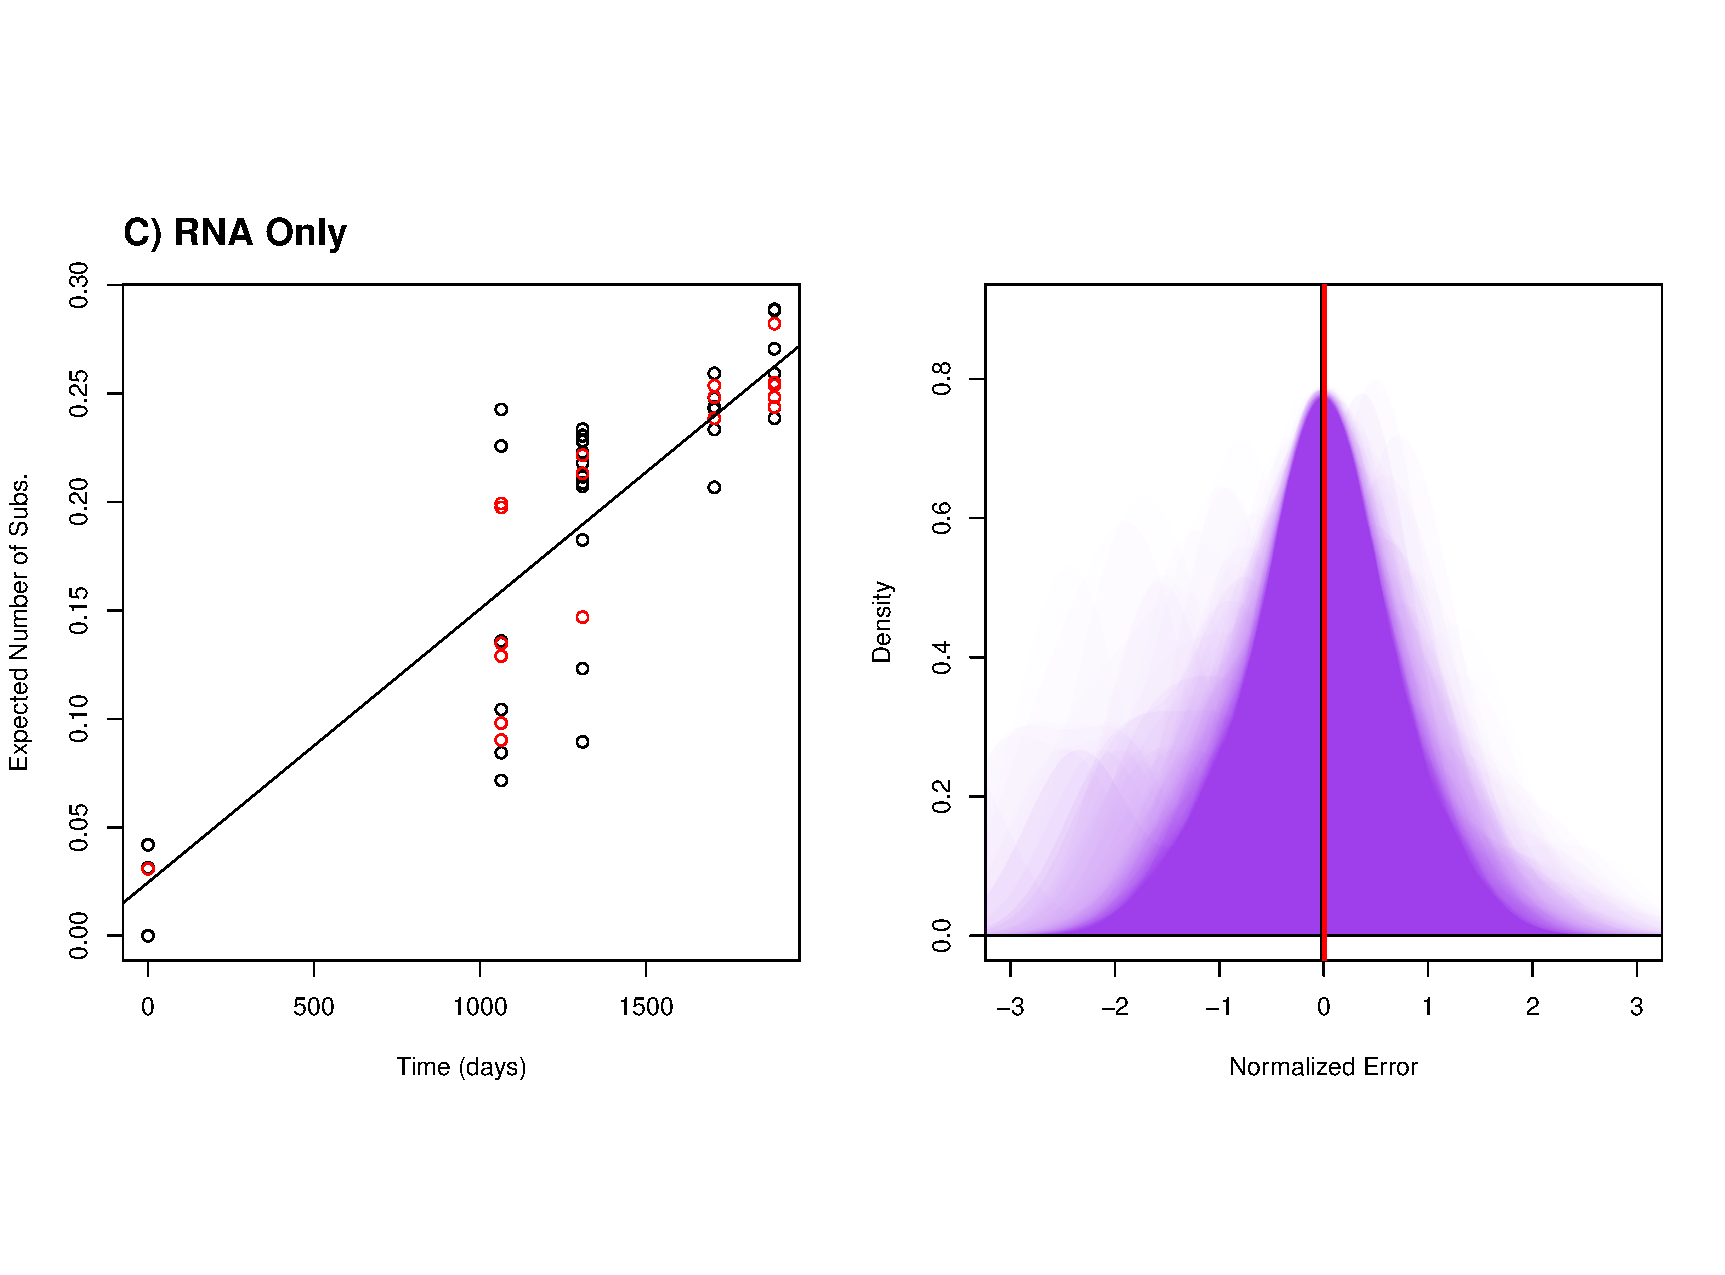
\includegraphics[trim=0cm 0cm 0cm 7cm, clip=true,scale=0.425]{figures/ancre.pdf}\\
	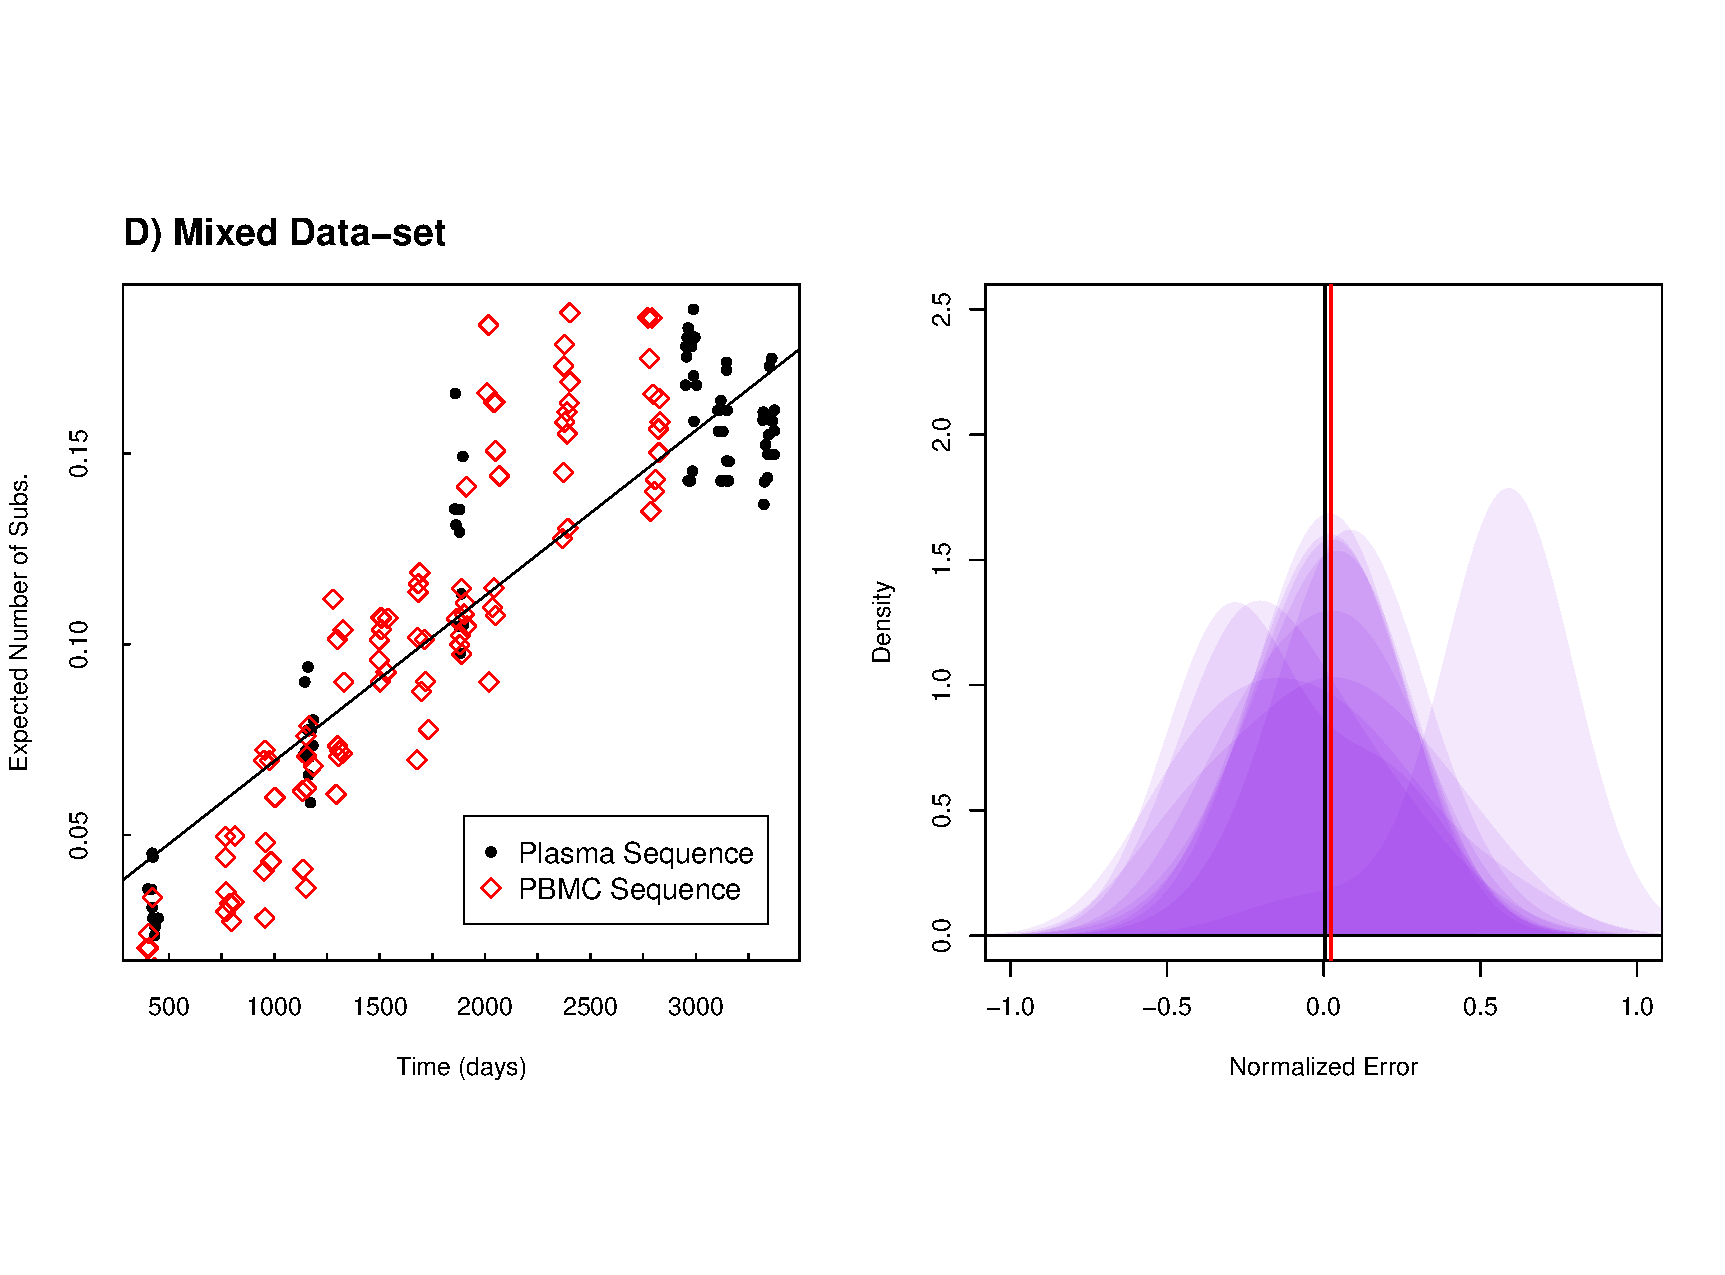
\includegraphics[trim=0cm 4cm 0cm 7cm, clip=true,scale=0.425]{figures/lanl.pdf}
	\caption[Examples]{\anote{Add legend, change points, change shading, explain point colouring, explain mean and median lines.}}
\end{figure*}


\subsection{Simulated Data} \label{sec:sim_results}
For our simulated data, we evaluated three error metrics. We looked at the mean square error for each synthetic tree, as well as the mean and median difference between the predicted date and sampling date. Figure \ref{fig:results1} A) shows that the clock is a reliable source of information in this case. Quantitatively, the censored data points are close to the regression line, and the difference density is heavily peaked around 0. Averaged over all simulated data sets, the average mean square error was \anote{X}, and the average median and mean difference were \anote{Y} and \anote{Z} respectively.

We evaluated the latent simulated data under similar metrics. Figure \ref{fig:results1} B) shows the regression over the calibration dates and the simulated collection dates. Note that these dates are not the actual. In this experiment, the density plot is shifted to the right, exemplifying latent behavior. Averaged over all simulated data sets, the average mean square error was \anote{X}, and the average median and mean difference were \anote{Y} and \anote{Z} respectively. However, when we utilized the known sample ages (as opposed to the collection dates) then measured the same metrics, averaged over all simulated data sets, the average mean square error was \anote{X}, and the average median and mean difference were \anote{Y} and \anote{Z} respectively.

\subsection{RNA Only Data} \label{sec:rna_only}
To evaluate the possible effectiveness of this methodology on real data, we utilized the plasma only data set \citep{McCloskey14}. For every applicable patient, we censored 50\% of their known sampling dates then reconstructed the censored dates using the linear model calibrated over the uncensored dates. We also performed this experiment with RTT rooting and out group rooting \anote{we should have another figure like figure 2 for both RTT and out-group rooting}. The goal of this experiment was to parallel the type of results from \ref{sec:sim_results}.

Figure \ref{fig:results1} C) shows the regression over the calibration dates and the collection date. Averaged over all simulated data sets, the average mean square error was \anote{X}, and the average median and mean difference were \anote{Y} and \anote{Z} respectively. The superposition of the difference density plots shows similar behavior to that of \ref{sec:sim_results}, except with a wider distribution, and more variation. Since there is inherently more noise in this data, this is expected. 

\subsection{Patient Reconstruction}
Finally, we looked at patients who had both plasma and PBMC samples available. We used both RTT and outgroup rooting to root the phylogeny, then calibrated a clock to the known plasma sampling dates and reconstructed the expected age of the sequences for all patients who could reject the null model \ref{subsec:hypot}. 

Figure \ref{fig:results1} D) shows the regression over the calibration dates and the simulated collection date. In this case, we do not know the actual date of archival.  The superposition of the difference density plots shows similar behavior to that of the latent simulated data, except \anote{need new plots for this}.  

The patients that had received treatment at some point generally failed the hypothesis testing -- there was only one patient that did not. This suggests that after a patient begins treatment, the assumption of a molecular clock over their phylogeny is too strong. 
